\chapter{BioScope: a Flexible and Extensible Wearable Platform}
This chapter presents the design and implementation of BioScope, a flexible and extensible wearable platform for rapidly prototyping healthcare applications (Figure \ref{bio_fig0}). BioScope is an extensible bandage system with components that can be stacked like Lego blocks. Using this system, users can simultaneously collect the four most commonly monitored biosignals (i.e., heart rate, body temperature, acoustic signals emitted from the body, and inertial readings of human movement) from multiple bandages to assess and diagnose physical conditions. BioScope extracts the processing and communication functions into a core building block, and hosts the required sensors. Each sensor is affixed as a patch that collects one biosignal. By stacking the required sensors onto a bandage-like platform, users can easily create a customized bandage that can be affixed to the skin of the patient. The data collected by the sensors are sent through a Bluetooth interface to the device screen used by the healthcare worker. 

\begin{figure}[!ht]
\centering
\includegraphics[width=14cm]{image/bio_fig0}
\caption{BioScope: a flexible and extensible wearable sensing platform. }
\label{bio_fig0}
\end{figure}


\section{Design Exploration}

The first step of iterative design for a wearable sensing platform is to understand the needs of potential users. We conducted two focus groups and two participatory design workshops to explore the needs from healthcare professionals.

\subsection{Focus Groups}
We conducted two focus groups to better understand the practical needs of wearable technology in clinical setting. In the first focus group, we recruited four nursing professionals and two physical therapists from National Taiwan University Hospital. In the second focus group, we recruited four nursing professionals from Taipei City Psychiatric Center (TCPC).

\subsubsection{Participants}
In the first focus group, we recruited four healthcare workers (four experienced nursing experts and two physiotherapists), aged from 27 to 46 years. The four experienced nursing experts had worked as registered nurses for more than three years and the two physiotherapists have worked in the Rehabilitation Department of National Taiwan University Hospital at least six years. These participants have prior experienced in oncology, cardiology, and orthopedics. Four experts in the second focus group, aged from 35 to 45 years, have worked as registered nurses for more than ten years at the Taipei City Psychiatric Center (TCPC) and specialized in providing inpatient psychiatric care for children, adolescents, geriatrics, and patients with substance abuse.

\subsubsection{Procedures}
The moderator of the focus group was a researcher with background in engineering. After explaining the objective of the focus group, we provide five mock-up wearable devices with different form factors to the participants. Then, the moderator asked their perceptions regarding the usability, safety, and potential applications of those form factors. The second topic of the focus group is to encourage stories with clinical scenarios that can reveal how wearable devices may benefit different healthcare applications.

\subsection{Participatory Design Workshops}
We conducted participatory design workshops to look for opportunities and constrains concerning the use of wearable sensing technologies in healthcare applications. Following the participatory design process \cite{Greenbaum:1992:DWC:125470, Muller:2002:PDT:772072.772138}, two workshops were held to co-design devices to assist healthcare workers in designing a wearable sensing platform.

\subsubsection{Participants}
Eight nursing professionals (four experienced nursing experts and four senior nursing school students), aged from 22 to 46 years, with experience in clinical nursing, were recruited. Four experienced nursing experts had worked as registered nurses for at least seven years and the four senior nursing school students had been nursing interns in hospitals for at least half a year. All participants were experienced in nursing patients in multiple medical divisions, with the main specialty spanning in divisions of oncology, pediatrics, cardiology, and orthopedics.

\subsubsection{Prior to a Workshop}
The nursing professionals were briefly introduced to the goal of this study and the structure of the workshop several days (about four to six days) prior to the workshop. Before attending the workshop, participants were asked to finish the pre-workshop homework similar to “homework” assignment to participants prior to each workshop in the PICTIVE project \cite{Muller:1991:PEP:108844.108896}. This pre-workshop homework involved a design sheet to help participants describe and/or sketch five potential ideas for designs of devices that used any related wearable sensing technology to assist them in resolving difficulties that they faced at work or in their daily life. Since the purpose of this pre-workshop homework was to encourage the participants to generate a wide range of designs in the workshop, the participants were not asked to evaluate the feasibility of their prototype devices for solving the described problems or to limit them in their focus on post-operative caring scenarios. This pre-workshop homework helped the participants to brainstorm a wide range of ideas and collect observations from their working or everyday life as a warm-up for the upcoming workshop.

\subsubsection{Procedures}
This workshop comprised of three sessions, which were (1) an engagement session, (2) a guiding session, and (3) a development session. Two participatory design workshops were held on two separate days. Each workshop lasted approximately four hours, including a half-an-hour break for lunch.

\textbf{Engagement session:} 
\newline
In the engagement session (which lasted for half of an hour), all participants introduced themselves and presented the five design ideas that they had prepared for their pre-workshop homework. While presenting a design idea, each participant stuck a design note that also described the idea on a white board. Researchers generated appropriate categories and grouped similar ideas as the participants were placing their notes. After all of the notes on the white board, researchers and participants discussed and moved the notes among categories or to a new category using the affinity diagramming method. All of the categories indicate potential directions or building blocks in the development of the solution in the final design of the workshop. 

\textbf{Guiding session:} 
\newline
In the guiding session (which lasted for half of an hour), a moderator, who was a researcher with an engineering background, introduced the sensing technologies or projects related to healthcare applications. The purpose of the workshop was explained to participants, which was to use wearable and/or environmental sensing technologies in the design of devices that can help healthcare workers in caring for post-operative patients in hospital. 

\textbf{Development session:} 
\newline
In the final developing session (which lasted two and a half hours), four participants were separated into two pairs in which each participant could share design opinions. To stir cross-disciplinary thinking within each pair, one researcher with an engineering background helped participants to identify alternative sensing technologies for use in their design work, and another researcher with a background in industrial and commercial design expressed their design scenarios using concrete storyboards. Consistent with the work-oriented participatory design process, the goal of each design was set, which was to help healthcare workers care for patients in hospitals. To assist participants in performing the design task effectively, an A3 sheet of paper with the following fields was provided; name of their solution, target user, needs of the target user, targeted sensing events and required feedback, form factor of the designed device. The first stage of the development session involved the participants discussing the name and the target user of the designed solution using categories that were obtained from the pre-workshop homework. Following the identification of the target users, the second stage involved determining the potential needs of the target user that are associated with the solution. In the third stage, the engineering researcher discussed with participants the selection of sensors and actuators for detecting targeted events or generating the required feedback in each application scenario. When the group completed its final design, the designer cooperated with the participants to finalize the form factor of the designed device by sketching an appropriate storyboard. In the final stage, each group presented their final design, about which all participants discussed and commented.

\subsection{Findings form Explorative Studies}
%In addition to medical-background users, a team to develop an application may involve cross-disciplinary members.
%The users with different background knowledge and skill levels have various requirements for prototyping. 
%To better understand the needs of engineering-background users, we further conduct semi-structure interviews on 6 participants, who have experience on HCI projects (4 male and 2 female age from 22 to 33 with computer science or electrical engineering background).
The design goal of BioScope towards a flexible and extensible platform that can fit in with different types of users. We describe the design considerations for both non-engineering background and engineering background users.

For data analysis, the audio recordings of focus groups and interviews, and the video recordings of the participatory design workshops were transcribed and coded.
With lessons learned from our study and observations, we summarize the findings of design exploration for developing a wearable sensing platform as follows.

\subsubsection{Findings}
\textbf{Form factor:}
\newline
Several wearable form factors are discussed to identify what are the nice characteristics as a wearable device, including wristband, neckband, sticker, bandage, badge, garment, flip flop, strap and so on. The explored characteristics include easy wearing, taking off, compact and comfortable. The device should be comfort to wear and quick to deploy. The device also can be placed on proper body location to sense physiological data.

\vspace{10pt}
\textbf{Flexibility:}
\newline
Because there are various types of physiological sensors that can be used to develop different healthcare applications, a fixed design can only to offer limited functions on a device. It is difficult to have one single design that can fit all requirements to develop healthcare application. Therefore, if a wearable sensing platform has flexibility that developers can build a wearable device with required sensing abilities. Then, developers can use this device as a prototype to test their tailored healthcare application. In different iterations of design process, a platform with flexibility can easily deal with the situation that developers may need to add or remove functions on the wearable device.

\vspace{10pt}
\textbf{Extensibility:}
\newline
A wearable sensing platform must be easily extend and upgrade its abilities. In terms of the hardware part, the platform must be able extend new component without re-design entire system. In terms of the software part, the platform must provide comprehensive APIs to allow users to construct new method, function and algorithm on top of existing components.

\vspace{10pt}
\textbf{Sensing and data:}
\newline
To develop a healthcare application, several types of common information are collected using wearable device, such as vital sign, physical activity and so on. Since a wearable device collects sensory data, the next step is to process the data. Then, the system can feedback the processed data to corresponding users depending on their requirement. The platform should provide a meaningful representation of data that can be understood by the user, e.g.: a pedometer shows step count rather than raw data of motion sensor.

\vspace{10pt}
\textbf{Configuration:}
\newline
The complexity of configuration is a key whether users will adopt a platform for developing their application or not. For non-engineering background users, they desire there is no complex steps to configure the device and the components are plug and play. For advanced developers, they would desire further customization on top of the platform to realize some specific functions and applications. 

\vspace{10pt}
\textbf{Battery life:}
\newline
The work period of the wearable device is a critical concern for a healthcare application. The device must be able to survive until its mission is complete. However, enabling power saving relies on correct configuration on both hardware and firmware. A proper power saving mechanism can prolong the work period of the wearable device as long as possible and can work transparently to the user without complex configuration.




\section{BioScope System Design and Implementation}
Based on the design considerations, we designed and implemented the BioScope system. The following subsections include (1) flexible and extensible sensing bandage, (2) stacking mechanism, (3) sensor patches, (4) explorative experiment.

\begin{figure}[!ht]
\centering
\includegraphics[width=14cm]{image/bio_fig1}
\caption{Design of the extensible sensing bandage. (a) Four patches with distinctive embossed icons are stacked on the inner and contact layers according to the direction indicated by the red dotted arrows. (b) The sound-collecting structure (box with red dashed border), a thermocouple wire (box with blue solid border), and two electrodes coated with a conductive gel (two green circles) directly contact the skin.}
\label{bandage_stacking}
\end{figure}


\subsection{Flexible and Extensible Sensing Bandage}
Based on the design considerations from our explorative studies for designing a flexible and extensible platform that can facilitate data collection, we collaborated with an expert from the Department of Nursing at National Taiwan University, Taipei, Taiwan. Through biweekly meetings with the expert, we first identified the necessity for an extensible sensing device that can assist healthcare workers in efficiently collecting commonly monitored data used in nursing assessments (e.g., monitoring the functional recovery of postoperational patients). Based on input and feedback provided by the expert and two experienced healthcare workers (three women, aged 30$\sim$42 years), we explored alternative designs for the flexible and extensible sensing device. During these brainstorming sessions, we recorded the ideas of all participants and then organized these ideas by using affinity diagrams to gain a deeper understanding of the primary design considerations.

The system should enable healthcare workers to tailor the sensors to specific assessments. Depending on the diagnostic results, healthcare workers may wish to reassess the patient by collecting additional data. The system should therefore enable preliminary screenings in which the healthcare workers can add or remove sensors to the device. For developer, the system should be able to extend new component without re-design entire system.

The system should be efficient and simple to use, even for healthcare workers with no technical background. After determining the types of data required for patient assessment, healthcare workers should be able to easily identify which sensors to add to the device. To enable healthcare workers to attach the required sensors to appropriate locations on the patient, the device should have a compact adhesive design, enabling it to be easily affixed to the skin without undue inconvenience or skin irritation \cite{Barrett2014}. 

The system should be able to analyze trends in data that are collected continually over durations ranging from several hours to several days. Healthcare workers can use this long-term data to review and reassess the physical state of patients and identify potential health complications. To continually collect data within a given period, (e.g., half of a day), a fully charged battery should contain sufficient energy to power the sensing device and the system should be able to enable power saving mechanism to prolong the battery life.

To create a flexible and extensible system, we designed a device with two distinct types of module (Figure \ref{bandage_stacking}): (1) the basic bandage platform and (2) sensor patches. The bandage-like platform resembles an adhesive bandage. We drew a 3D model of the platform and then printed it using a 3D printer and elastic filaments. Figure \ref{bandage_stacking}(a) depicts the platform, in which a hollow space is reserved to encase the customized sensing patches. To provide processing and communication capabilities, we designed a customized circuit board, called the main board, that could be mounted in the hollow space. The main board and the stacked sensor patches are powered by a 130-mAh Li-ion battery situated in the upper layer of the platform. On the main board, a Microchip PIC32MX150 microcontroller receives data from the sensor patches through board-to-board connectors, and then relays the processed data to the monitoring screen through a Texas Instruments CC2451 microcontroller with Bluetooth radio. 

\begin{figure}
\centering
\includegraphics[width=15cm]{image/bio_stack}
\caption{Stacking mechanism to connect sensor patches and mainboard.}
\label{bio_stack}
\end{figure}

\subsection{Stacking Mechanism}
Users can choose different combinations of LEGO-like sensing and interaction blocks and assemble them inside a bandage form factor. The key mechanism that enables BioScope to be flexible and extensible is stacking (Figure \ref{bio_stack}). In this subsection we We define a connecting protocol to unify the power supply and data communication between the patches and the mainboard. 

\vspace{15pt}
\subsubsection{Assembling}
Figure \ref{bio_steps}(a) illustrates these patches stacked in two layers in the hollow space of the platform; temperature and microphone sensors directly contact the skin to collect high-quality signals. 
To create accessible patches for the users, each patch was punched with a representative icon on both sides of the covering material. Figure \ref{bio_steps} illustrates the BioScope application process: (1) A healthcare worker selects the appropriate patches (or dummy patches) by using the embossed icon as a reference, stacks the patches on (or filling in empty spaces that are originally occupied by unused patches on) the platform, (2) inserts a battery and closes the protection cap, (3) affixes the bandage to chest, and (4) covers the entire bandage with transparent film dressings if water-proof is needed.

\begin{figure}
\centering
\includegraphics[width=15cm]{image/bio_fig2}
\caption{Four steps for applying bandages.}
\label{bio_steps}
\end{figure}


\begin{figure}
\centering
\includegraphics[width=15cm]{image/bio_dc_adc}
\caption{An example of using BioScope to prototype a breathalyzer.}
\label{dc_adc}
\end{figure}

\vspace{10pt}
\subsubsection{Power source}
Each component in the system may require various power supply range. Since a component may require a supply voltage higher or lower than the voltage from li-ion battery (4.2V), the voltage of power source should be converted to proper voltage. A linear regulator can be used to lower the power source to the working supply voltage. The mainboard equips a Microchip MIC5392 regulator with two 3V outputs, one output supplies the microcontroller and another output supplies peripheral patches that can be turned on/off by microcontroller. If the supply voltage of a component is higher than power source, a DC-DC converter can converts the voltage to a higher voltage. In figure \ref{dc_adc}, the supply voltage of the gas sensor is 5V which is higher than the voltage of the battery. Therefore, we place a compact DC-DC convertor, a Texas Instruments TPS81256, to boost the voltage to 5V and provide sufficient current to enable the sensor.
A compact switch button is mounted on the mainboard used to wake-up and reset the system. For power saving purpose, the system must be able to enter low frequency mode which only can be waked up by external interrupt. All peripheral components and radio frequency function can not work in low power mode. Also, the system will scan plugged patches when reset is triggered and wait the command from terminal device, i.e., mobile phone. 

\vspace{10pt}
\subsubsection{Data communication}
For a sensor that communicate to the microcontroller through digital bus, I2C and SPI are two most common protocols. Those protocols is bus topology that allows microcontroller can access multiple slave components with only few pins. SPI requires slave select pin to enable particular slave component for communication, our first prototype supports up to three salve components. 

However, some sensors are designed to output analog signals to deliver sensory data rather than digital signals. In Figrue \ref{dc_adc}, a Texas Instruments ADS1114 analog-to-digital converter translates the analog signals from gas sensor to digital signals in I2C. Thus, the system doesn't have to provide multiple pin-to-pin analog channels to serve individual analog sensor. 

\vspace{10pt}
\subsubsection{Horizontal expansion}
In addition to vertical stacking (Figure ?), the system provide horizontal expansion supported by a tiny H-bridge board (Figure ?), which has two sets of plug and receptacle connectors. The H-bridge board can be connected on plug connector or receptacle connector on the top or button of the board (Figure ?). For advanced developers, they may need to connect a component the system doesn't support. A breakout board (Figure ?) can be use to test new component for developing new patch for BioScope platform. The developer can evaluate customized component as well as off-the-shelf development toolkit.

\subsection{Patches}
To collect biosignals, such as electrocardiogram (ECG) signals, two pre-allocated electrodes (i.e., two conductive copper areas situated 6.4 cm apart at opposite ends of the bandage) are coated with a thin layer of electrical gel (Figure \ref{bandage_stacking}(b)).
The sensor patches, consisting of small sensor boards sandwiched between two thin layers of 3D-printed elastic filaments, are mounted on the bandage-like platform using connectors. To demonstrate the concept of this system, we designed six types of patch — biopotential, thermal, acoustic, mobility, interaction and recharging patches — to facilitate the collection in the most commonly monitored data in healthcare applications.
The detail of those six types of patch are described in follows.
\vspace{15pt}
\newline 
\textbf{Biopotential patch:}
\newline
This 23 mm × 24 mm patch, stacked in the inner layer, amplifies and filters ECG signals to enable continual cardiovascular monitoring. Cardiac activity, which can be characterized by ECG signals, is a crucial biosignal for assessing the cardiac functions of people. By amplifying the electrical potential difference measured between the two electrodes by using a Texas Instruments ADS1115 analog-to-digital converter on the patch, ECG signals can be monitored by allowing the passing of low-frequency signals from 0 to 100 Hz \cite{shaikh1995} by using a low-pass filter. A pulse can be identified by detecting spikes in the signal, thus enabling users to assess heart and respiratory rates.
\vspace{10pt}
\newline
\textbf{Acoustic patch:}
\newline
This 24 mm × 24 mm patch, stacked in the contact layer, records acoustic signals emitted by a person's body or while the person is phonating. By identifying the unique sound patterns that the body's organs generate, users can assess person's conditions. Furthermore, person's phonation can indicate social interaction, according to which users can assess whether a person is depressed or impaired cognitively.  To clearly record the internal sounds of the body, a mediating instrument (e.g., a stethoscope) is required. Inspired by the design of electronic stethoscopes, we designed and attached a small sound-collecting structure (Figure \ref{bandage_stacking}(b)) on the patch that effectively amplified acoustic signals from the body and occluded environmental noise. Above the sound-collecting structure, an opening is aligned with the receiving hole of an InvenSense INMP441 microphone with I2S interface on the board to guide sound waves towards the hole. In this study, we detected a person phonation, which reflected social activity, by analyzing the frequency components of the collected sound.
\vspace{10pt}
\newline
\textbf{Thermal patch:}
\newline
This 10 mm × 24 mm patch is stacked in the contact layer and measures the skin temperature, which can indicate a person's health. users can evaluate a person by identifying abnormal or varying temperatures \cite{Freitas1999}. A Maxim MAX31850 K-type thermocouple-to-digital converter detects body temperature through a thermocouple wire that protrudes from the covering elastic material to contact the skin of the person (Figure \ref{bandage_stacking}(b)).
\vspace{10pt}
\newline
\textbf{Mobility patch:}
\newline
This 11 mm × 24 mm patch, stacked in the inner layer, monitors the mobility level of a person. For example, to prevent complications caused by reduced mobility levels and assess functional recovery, users must track the mobility level of patients. On this patch, an InvenSense MPU6050 6-axis motion sensor is used to collect motion readings, which indicate whether a person is moving or stationary. The mobility level can be derived by calculating the percentage of time a person is moving.


\begin{figure}
\centering
\includegraphics[width=14cm]{image/bio_fig1_5}
\caption{Interaction patch includes OLED display and on-the-air gesture sensor}
\label{interaction_patch}
\end{figure}


\textbf{Interaction patch:}
\newline
To enrich data feedback and user interaction for exercise applications, we also expanded an interaction patch (Figure \ref{interaction_patch}) that consists of a tiny display (0.96” OLED display), and a touchless gesture sensor (Avago APDS-9960) that is used to recognize six directions (near, far, up, down, left and right) of on-the-air swipe gesture. The gesture can be used to switch between different sensor's data or different data representations. The interaction patch is connected to main board through stacking mechanism as well. When a mobile device attempts to establish connection with particular one of multiple wearable devices. To simplify Bluetooth pairing procedure for quickly retrieving data or configuring device, a NXP NTAG203 NFC tag is embedded in wearable device.
\vspace{10pt}
\begin{figure}[ht]
\centering
\includegraphics[width=13cm]{image/bio_recharge}
\caption{Recharging patch.}
\label{bio_recharge}
\end{figure}
\newline
\textbf{Recharging patch:}
\newline
The entire system is powered by a Li-ion battery with 130-mAh capacity. This patch has a USB connector to connect a 5V power source for charging and a Texas Instruments BQ24040 to regulate the voltage in charging process (Figure \ref{bio_recharge}).

\subsection{Explorative Experiment}
To validate system functionality, we scripted a sequence of activities to simulate conditions arising when a patient with basic functional mobility is hospitalized. Two volunteers performed the specific activities while wearing bandages equipped with all four patches on their chests, enabling us to collect data (Figure \ref{bio_exp_result}(a)). The simulations were con- ducted for 10 and 30 minutes in the cases of the first and second participants (P1 and P2), respectively. Activities comprised (1) lying down on a bed, (2) having a phone conversation, (3) watching TV, (4) having a face-to-face conversation, and (5) performing walking. In the experiments, the data captured were heart rate, skin temperature, received acoustic signals, and mobility indicators.


\begin{figure}[!ht]
\centering
\includegraphics[width=12cm]{image/bio_fig4}
\caption{Four steps for applying bandages.}
\label{bio_exp_result}
\end{figure}


Figure \ref{bio_exp_result}(b) shows the results obtained by analyzing the data collected from P1. The readings obtained from the mobility patch indicated that P1 moved between the seventh and ninth minutes; this was an accurate assessment of the patient's behavior during that time. While walking, P1's heart rate increased relative to that while stationary between the start and the seventh minute. When the posture of the patient drastically changed, such as when P1 stood up near the second, seventh, and ninth minutes, the ECG signals were distorted \cite{chan2013}, producing a dip in the calculated heart rate. The sounds generated by clothes rubbing against the bandage when P1 moved adversely affected the quality of detected internal sounds, causing the amplitudes to increase between the seventh and ninth minutes. After filtering out sounds generated by movement, however, we could still detect when P1 phonated between the second and seventh minute. Based on the vocal resonance of the body \cite{Dacre2002}, we detected phonation by identifying the frequency components of sounds higher than the 0- to 3-kHz frequency range of the human voice [7]. Finally, the body temperature varied minimally (34$^{\circ}$C $\sim$ 35$^{\circ}$C) and was near the normal skin temperature of the human chest \cite{Freitas1999}. Overall, the results accurately reflected the activities performed by the participants.

To examine whether the system can detect reasonable values for the average heart rate, total moving duration, average skin temperature, and total phonating time, we analyzed the data collected from P2 over 30 minutes. The total moving duration was determined to be 7.2 minutes (actual value: 6.9 minutes), with an error of 4.0\%. The average heart rate was 81.5 and 100.3 beats respectively.  Because P2 did not perform intensive exercise, the average temperature did not vary significantly, remaining near 33.9◦C. By identifying the high-frequency components embedded in the high-pitched sounds collected when P2 was stationary, P2 was deter- mined to have phonated for 635.5 seconds (actual value: 564.0 seconds), with an error of 12.7\%. per min (BPM) when P2 was stationary and moving, respectively.  Because P2 did not perform intensive exercise, the average temperature did not vary significantly, remaining near 33.9◦C. By identifying the high-frequency components embedded in the high-pitched sounds collected when P2 was stationary, P2 was deter- mined to have phonated for 635.5 seconds (actual value: 564.0 seconds), with an error of 12.7\%.

%\subsection{Summary}
%In this section, we describe the hardware architecture to demonstrate the design concept of BioScope that provide flexibility and extensibility to fit in with different users' needs. 


%\section{Configuration}

%\section{Application programming interface}

\section{Visualization of Sensory Data}
The hardware design of BioScope sensing platform enables flexibility and extensibility, its firmware and software have corresponding design consideration to promote the prototyping phase of design process. This section describes the visualization of sensory data that allows users can simply receive raw and/or primitive processed data from sensors. Visualization is an efficient way that can assist users to easily understand the characteristics of sensors. 
In order to simplify the usage of the system for non-engineering background users, BioScope platform provides the basic mechanisms provided by BioScope platform to visualize sensory data: (1) display on interaction patch and (2) display on mobile device. The users can simply stacks needed patches on the mainboard of BioScope. The default firmware can detect attached patches and run corresponding process to collect sensory data and provide feedback.

\begin{figure}
\centering
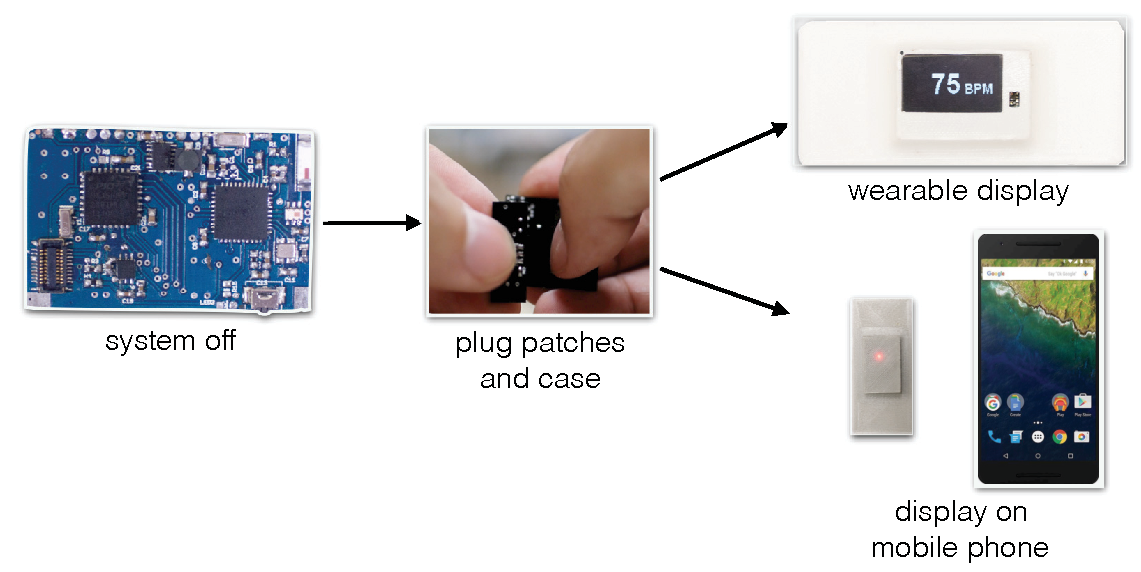
\includegraphics[width=15cm]{image/fig_config.ps}
\caption{The steps of configuration for data visualization. (a) System off. (b) Assembly: stacking patches and casing. (c) display on interaction patch. (d) display on mobile phone.}
\label{fig_config}
\end{figure}

\subsection{Configuration}
BioScope platform allows users to easily configure the system for collecting sensory data and receiving feedback from chosen patches with simple steps. We provide a mobile app running on top of Android for data configuration and data visualization. 
The main steps of configuration for data visualization is shown in Figure \ref{fig_config}. 

\subsubsection{System off} 
This is the initial state of the system, when the device is not applied a power source, i.e., install/recharge battery, or user configures the device to turn off the device.
As well as many off-the-shelf electronic products, the device doesn't have an on/off switch to shutdown the device. 
Instead, the system will enter to low power mode, because the consumed current in low power mode is negligible ($\sim$16 uA). 
The device will be turned to system off mode caused by two conditions: (1) pressing reset button on the device then idle for one minute, and (2) receiving the off command from mobile phone.
In low power mode, the microcontroller switches to secondary oscillator with low system frequency (32.768kHz) and turns off all internal components of the microcontroller for power saving. The device can only be waked up by external interrupt in system off mode.

\subsubsection{Assembly: Stack patches and casing} 
User can choose needed sensor patches and components to construct a customized device by simply stacking patches on the mainboard. Then the device is placed into a 3D printing case with the elastic filaments, e.g., bandage case.
When the device is booted, the system will blink the on-board LED and scan stacked patches on the mainboard through I2C and SPI bus. For the patches with I2C bus, the system will query the specific addresses defined in the BioScope system to check whether the patch is attached. For the patches with SPI bus, the system will query the connected patch by setting each slave select pin to high voltage individually. Thus, the system can automatically determine attached patches without users' effort to manually input the chosen patches.

\subsubsection{Display data}
The mobile phone is used as a terminal for configuring device and visualizing sensory data via Bluetooth radio.
The mobile phone is the central and the BioScope device is peripheral in the wireless topology.
After stacking the chosen patches and casing, user can use the mobile phone to establish the connection with device.
Then user can configure the mobile phone to display sensory data on the screen.

The device can also operate without communication with the mobile phone.
When the interaction patch is detected on the I2C bus, the system will run the corresponding process for basic sensing and feedback functions with wearable display.
Users can switch and control the displayed sensory data through the touchless gesture sensor on the interaction patch.
The system also allows the device to be further configured and accessed through the user interface on mobile phone as well.

\begin{figure}
\centering
\includegraphics[width=14cm]{image/fig_represent.eps}
\caption{Representations of data visualization on wearable display: digit, pattern, icon.}
\label{fig_represent}
\end{figure}

\subsection{Data Processing and Representation}
Considering application need, wireless bandwidth and power efficiency, the sensory data should be processed in different ways.
For example, the device transmits raw data of ECG to mobile phone for further computation that requires a sampling rate of 200 Hz (400 bytes per second). 
Such high data rate will consume a lot of power for data transmission.
If the application needs heart rate data rather than the raw data of ECG, the device can determine every single peak of the raw data for computing average heart rate and than transmit data with sampling rate of 1 Hz (1 byte).
Thus, the overall power consumption can be significant reduced by processing data using the microcontroller.
However, the microcontroller may not be able to compute high complexity work, e.g., activity recognition with motion data.
For this case, developers have to adopt higher performance processor or transit raw data to mobile phone for processing.

The data can be illustrated in different representations for visualization depending on users' needs.
For example, displaying heart rate data with interaction patch can be different representations: (1) digit: beats per minute, (2) pattern: raw data and (3) icon: blink with beat (Figure \ref{fig_represent}).


\subsection{User Interface on Mobile Device}
The mobile device is versatile and pervasive in our daily life.
Therefore, we built a mobile app running on top of Android platform to facilitate data visualization and device configuration.
\vspace{10pt}
\newline
\textit{Device scan:}
\newline
The first page (Figure ? (?)) of the mobile app shows the BioScope devices nearby. The device without specific prefix in device ID is filtered out. By pressing the particular device in the list, the system will start to establish the connection with the device.
\vspace{10pt}
\newline
\textit{Attached patches:}
\newline
When the connection between phone and device is established, the mobile app will list all attached patches on the screen (Figure ?(?)).
\vspace{10pt}
\newline
\textit{Select function:}
\newline
A patch may have multiple functions, user can configure and visualize the data of each function separately (Figure ?(?)).
If the check button of each function in the list is checked, the sensory data will be logged in the storage of mobile device.
User can export these log data to PC for further analysis.
\vspace{10pt}
\newline
\textit{Config visualization:}
\newline
By choosing a function in the list, the data is visualized on the screen of the mobile phone. User can further config the data and its representations (Figure ?(?)).


\section{Platform APIs}
In previous section, we introduced the basic data visualization and collection on BioScope platform that enables plug-and-play stacking mechanism and easy-to-use interface.
In addition to visualizing and collecting data, advanced developers may need to further program the system for building their own application.
We provides device APIs and phone APIs to facilitate building application on BioScope platform.
The device APIs allow developers to simply access the sensors and Bluetooth radio on BioScope device and phone APIs to retrieve sensory data and configure device on the smart phone. 

\begin{figure}
\centering
\includegraphics[width=12cm]{image/mcu_codes.eps}
\caption{Extract the initialization and loop sections from conventional structure of microcontroller codes}
\label{fig_mcu_codes}
\end{figure}

\subsection{Device APIs}
The BioScope system adopts a Texas Instruments CC2451 microcontroller as the core of the wearable device.
However, the software developing environment of microcontroller may be too complicated for the users.
To facilitate the access of components on BioScope platform, we encapsulates the detail codes to the APIs based on the software stack provided by Texas Instruments.
As well as the prototyping platforms in the market, we extract the initialization and loop sections from conventional structure of microcontroller codes (Figure \ref{fig_mcu_codes}).
Thus, developers only need to handle initialization and periodical routine and  callback events.

\begin{figure}[ht]
\centering
\includegraphics[width=11cm]{image/mcu_temp.eps}
\caption{An example of BioScope device APIs for reading temperature sensor and transmitting sensory data through Bluetooth radio}
\label{fig_mcu_temp}
\end{figure}

Figure \ref{fig_mcu_temp} shows an example for reading data from temperature sensor and transmitting sensory data through Bluetooth radio.
In \textit{BioScope\_init} function, developers only need to declare the struct variables of Bluetooth component and temperature sensor. And the configuration of the loop interval must be set up in the initialization section for power sensing requirement.
Then the \textit{BioScope\_loop} function runs sensory reading and radio transmission periodically with the specific interval.
The provided APIs in C language are summarized as follows.

\subsubsection{System}
\textit{uint16\_t* getPatchList()}: Get the list of attached patches on the device.
\vspace{10pt}
\newline
\textit{void setLoopInterval(uint16\_t interval)}: Set the interval(ms) of the loop.
\vspace{10pt}
\newline
\textit{void setLoopIntervalSec(uint16\_t interval)}: Set the interval(sec) of the loop.
\vspace{10pt}
\newline
\textit{void delayMS(uint16\_t ms)}: Delay for the number of millisecond.
\vspace{10pt}
\newline
\textit{void delayUS(uint16\_t us)}: Delay for the number of microsecond.
\vspace{10pt}
\newline
\textit{void enablePowerSaving()}: Enable power saving. If idle, the system will turn to low-power mode until next interrupt occurs.
\vspace{10pt}
\newline
\textit{void disablePowerSaving()}: Disable power saving. The processor stays in fastest frequency and all peripheral components are enabled as well.
\newline

\subsubsection{Sensor}
\textit{bool isAttached(uint8\_t patch)}: Determine whether a patch is attached on the device or not.
\vspace{10pt}
\newline
\textit{void detached(uint8\_t patch)}: The callback function is invoked when a patch is detached.
\vspace{10pt}
\newline
\textit{uint16\_t readTemp()}: Read temperature data from thermal patch.
\vspace{10pt}
\newline
\textit{uint16\_t readHeartRate()}: Read heart rate from Biopotential sensor.
\vspace{10pt}
\newline
\textit{uint16\_t* readAccelerometer()}: Read 3-axis accelerometer data from mobility sensor.
\vspace{10pt}
\newline
\textit{uint16\_t* readGyro()}: Read 3-axis gyro data from mobility sensor.
\vspace{10pt}
\newline
\textit{uint16\_t* readMagnetic()}: Read 3-axis magnetic data from mobility sensor.
\vspace{10pt}
\newline

\subsubsection{Interaction patch}
\textit{void writeChars(uint8\_t *chars, uint8\_t size)}: Write characters on the OLED display with specific size.
\vspace{10pt}
\newline
\textit{void drawIcon(uint8\_t *icon)}: Draw an icon on the OLED display represented by bitmap format.
\vspace{10pt}
\newline
\textit{void isGesture(uint8\_t gesture)}: Check whether a specific gesture is detected.
\vspace{10pt}
\newline
\textit{void gesture(uint8\_t gesture)}: The callback function is invoked when a gesture is detected.
\vspace{10pt}
\newline

\subsubsection{BluetoothLE radio}
\textit{void bleConnected(uint8\_t *centralAddress)}: The callback function is invoked when a central device has connected with this device.
\vspace{10pt}
\newline
\textit{void bleDisconnected(uint8\_t *centralAddress)}: The callback function is invoked when a central device has disconnected with this device.
\vspace{10pt}
\newline
\textit{void send(uint8\_t type, uint8\_t  length, uint8\_t *data)}: Send data to central device trough Bluetooth radio.
\vspace{10pt}
\newline
\textit{void received(uint8\_t type, uint8\_t  length, uint8\_t *data)}: The callback function is invoked when received a command from central device trough Bluetooth radio.
\vspace{10pt}
\newline

\subsection{Phone APIs}
The BioScope system provides APIs on Android platform for collecting sensory data and accessing the BioScope device.
The phone APIs consists of two classes: \textit{BioScopeBle} and \textit{BioScopeBleListener}.
The \textit{BioScopeBle} is the class that provides the functions to communicate with BioScope device through Bluetooth radio.
The \textit{BioScopeBleListener} is the interface class that allows developers to implement the callback functions of communication with BioScope device in their codes. The provided APIs in Java language are summarized as follows.

\subsubsection{BioScopeBle}
\textit{BioScopeBle(String device)}: The constructor of the class is used to new an object for communicating with specific BioScope device.
\vspace{10pt}
\newline
\textit{void connect()}: Start to establish connection with the BioScope device.
\vspace{10pt}
\newline
\textit{void disconnect()}: Disconnect an existed connection with the BioScope device.
\vspace{10pt}
\newline
\textit{void writeCharacteristic(int type, byte[] command)}: Write the command to a characteristic on the BioScope device.
\vspace{10pt}
\newline
\textit{int[] getPatchList()}: Get the list of attached patches on the BioScope device.
\vspace{10pt}
\newline

\subsubsection{BioScopeBleListener}
\textit{void bleNotSupported()}: The callback function is invoked if BLE is not supported in this device.
\vspace{10pt}
\newline
\textit{void bleConnectionTimeout()}: The callback function is invoked when the connection establishment is timeout (10 sec).
\vspace{10pt}
\newline
\textit{void bleConnected()}: The callback function is invoked when the connection establishment is success.
\vspace{10pt}
\newline
\textit{void bleDisconnected()}: The callback function is invoked when the established connection is disconnect.
\vspace{10pt}
\newline
\textit{void bleWriteSuccess()}: The callback function is invoked when the execution of the \textit{writeCharacteristic} method is success.
\vspace{10pt}
\newline
\textit{void bleWriteStateFail()}: The callback function is invoked when the execution of the \textit{writeCharacteristic} method is fail.
\vspace{10pt}
\newline
\textit{void bleDataReceived(int type, byte[] data)}: The callback function is invoked when the data sent from BioScope device are received.
\vspace{10pt}
\newline

\section{Summary}
In this chapter, we introduced BioScope, a flexible and extensible wearable platform designed to facilitate rapidly prototyping of the design process.
Users can choose the needed components to build a customized device for their application.
The system provides visualization of sensory data that users can simply access various primitive representations of sensory data.
The platform APIs allows advanced users to program the system to meet their requirement.
Users can therefore easily create a high-fidelity prototype for evaluating and testing required functions in their design.

\let\cleardoublepage\clearpage